\begin{savequote}[75mm]
Add your quote here
\qauthor{Author of quote}
\end{savequote}

\chapter{Literature Review}
\label{literature}
\newthought{Lorem ipsum dolor sit amet}, consectetur adipiscing elit. Nunc neque massa, eleifend malesuada enim eu, efficitur imperdiet nulla. Aliquam augue est, lobortis eget scelerisque at, pretium vel lorem. Etiam faucibus nulla quam, nec tristique elit ullamcorper quis. Phasellus vel tincidunt nisl. Mauris at lacus sit amet mi auctor feugiat. Donec vel maximus erat. Suspendisse feugiat augue lacus, non egestas libero auctor sit amet. Nunc eros ante, posuere quis justo id, congue ultrices sapien.

\clearpage


\section{Machine Learning}
%Nulla fringilla eu eros nec tempor. Phasellus volutpat nulla a lectus pulvinar, sit amet maximus ex semper. Fusce sagittis ligula magna, non condimentum lectus imperdiet ut. Nunc dignissim turpis nibh, vel tristique tellus tristique eu. Fusce posuere dictum ultricies. Nam a metus quis mauris gravida laoreet.

\subsection{Neural Networks}
%Nulla fringilla eu eros nec tempor. Phasellus volutpat nulla a lectus pulvinar, sit amet maximus ex semper. Fusce sagittis ligula magna, non condimentum lectus imperdiet ut. Nunc dignissim turpis nibh, vel tristique tellus tristique eu. Fusce posuere dictum ultricies. Nam a metus quis mauris gravida laoreet.

%Vivamus placerat tortor a egestas sollicitudin. Nulla fringilla eu eros nec tempor. Phasellus volutpat nulla a lectus pulvinar, sit amet maximus ex semper. Fusce sagittis ligula magna, non condimentum lectus imperdiet ut. Nunc dignissim turpis nibh, vel tristique tellus tristique eu. Fusce posuere dictum ultricies. Nam a metus quis mauris gravida laoreet. Fusce lacinia justo dui, ut ornare tortor pharetra consequat.

\subsection{Deep Learning}
%Nulla fringilla eu eros nec tempor. Phasellus volutpat nulla a lectus pulvinar, sit amet maximus ex semper. Fusce sagittis ligula magna, non condimentum lectus imperdiet ut. Nunc dignissim turpis nibh, vel tristique tellus tristique eu. Fusce posuere dictum ultricies. Nam a metus quis mauris gravida laoreet.

%Lorem ipsum dolor sit amet, consectetur adipiscing elit. Nunc neque massa, eleifend malesuada enim eu, efficitur imperdiet nulla. Aliquam augue est, lobortis eget scelerisque at, pretium vel lorem\footnote[2]{Vivamus placerat tortor a egestas sollicitudin. Nulla fringilla eu eros nec tempor. Phasellus volutpat nulla a lectus pulvinar, sit amet maximus ex semper. Fusce sagittis ligula magna, non condimentum lectus imperdiet ut.}. Etiam faucibus nulla quam, nec tristique elit ullamcorper quis. Phasellus vel tincidunt nisl. Mauris at lacus sit amet mi auctor feugiat. Donec vel maximus erat. Suspendisse feugiat augue lacus, non egestas libero auctor sit amet. Nunc eros ante, posuere quis justo id, congue ultrices sapien.


\subsection{Keras}
%Vivamus placerat tortor a egestas sollicitudin. Nulla fringilla eu eros nec tempor. Phasellus volutpat nulla a lectus pulvinar, sit amet maximus ex semper. Fusce sagittis ligula magna, non condimentum lectus imperdiet ut. Nunc dignissim turpis nibh, vel tristique tellus tristique eu. Fusce posuere dictum ultricies. Nam a metus quis mauris gravida laoreet. Fusce lacinia justo dui, ut ornare tortor pharetra consequat.



\section{Machine Translation}
\label{Machine Translation}


\subsection{Training Data}
%Nulla fringilla eu eros nec tempor. Phasellus volutpat nulla a lectus pulvinar, sit amet maximus ex semper. Fusce sagittis ligula magna, non condimentum lectus imperdiet ut. Nunc dignissim turpis nibh, vel tristique tellus tristique eu. Fusce posuere dictum ultricies. Nam a metus quis mauris gravida laoreet.

\subsection{Techniques}

\subsubsection{Rule-Based Machine Translation}
%Nulla fringilla eu eros nec tempor. Phasellus volutpat nulla a lectus pulvinar, sit amet maximus ex semper. Fusce sagittis ligula magna, non condimentum lectus imperdiet ut. Nunc dignissim turpis nibh, vel tristique tellus tristique eu. Fusce posuere dictum ultricies. Nam a metus quis mauris gravida laoreet.

\subsubsection{Statistical Machine Translation}
%Nulla fringilla eu eros nec tempor. Phasellus volutpat nulla a lectus pulvinar, sit amet maximus ex semper. Fusce sagittis ligula magna, non condimentum lectus imperdiet ut. Nunc dignissim turpis nibh, vel tristique tellus tristique eu. Fusce posuere dictum ultricies. Nam a metus quis mauris gravida laoreet.

\subsubsection{Transfer-Based Machine Translation}
%Nulla fringilla eu eros nec tempor. Phasellus volutpat nulla a lectus pulvinar, sit amet maximus ex semper. Fusce sagittis ligula magna, non condimentum lectus imperdiet ut. Nunc dignissim turpis nibh, vel tristique tellus tristique eu. Fusce posuere dictum ultricies. Nam a metus quis mauris gravida laoreet.


\subsubsection{Neural Machine Translation}
%Nulla fringilla eu eros nec tempor. Phasellus volutpat nulla a lectus pulvinar, sit amet maximus ex semper. Fusce sagittis ligula magna, non condimentum lectus imperdiet ut. Nunc dignissim turpis nibh, vel tristique tellus tristique eu. Fusce posuere dictum ultricies. Nam a metus quis mauris gravida laoreet.

\subsection{Evaluation}
%Nulla fringilla eu eros nec tempor. Phasellus volutpat nulla a lectus pulvinar, sit amet maximus ex semper. Fusce sagittis ligula magna, non condimentum lectus imperdiet ut. Nunc dignissim turpis nibh, vel tristique tellus tristique eu. Fusce posuere dictum ultricies. Nam a metus quis mauris gravida laoreet.

\clearpage

\section{Low-Resource Neural Machine Translation Approaches}
\label{LRNMT}

\subsection{Transfer Learning}

As outlined by \cite{torrey_transfer_2009}, transfer learning is able to use the knowledge gained from a previous task in order to improve model performance in a related task.
In a neural machine translation context, this involves training a model using data from a high-resource language and then using that model for initialising the model the will be trained on the low-resource language training data. This was demonstrated in research carried out by \cite{zoph_transfer_2016}, where transfer learning improved the performance of \acrshort{NMT} models for low-resource languages by an average of 5.6 \acrshort{BLEU} on four different language pairs. Results of the experiment also suggest that selecting a high-resource language closely related to the low-resource language can improve transfer learning models and therefore translation quality.

However, this contradicts more recent research by \cite{kocmi_trivial_2018}, which looked at "trivial transfer learning". Whereas existing transfer learning methods require a degree of language relatedness, trivial transfer learning prioritises data quantity for the high-resource language. Their findings indicate that the relatedness of the language pair is of less importance than the quantity of data used in the initial high-resource language training. Despite being unable to pinpoint the exact reasoning behind the improvement in results, they state that "our observations indicate that the key factor is the size of the parent corpus rather than e.g. vocabulary overlaps."
It is worth noting that \cite{kocmi_trivial_2018} use a transformer neural network architecture instead of the recurrent neural network architecture used by \cite{zoph_transfer_2016}. Research by \cite{popel_training_2018} found that using the transformer model leads to better translation quality, likely contributing towards the contradictory results.


Hierarchical transfer learning seeks ensure the closeness of the related language pair, as identified in most transfer learning research, while simultaneously addressing the importance of the high-resource data quantity outlined in trivial transfer learning. \cite{luo_hierarchical_2019} achieve this by implementing three distinct stages of training:

\begin{itemize}
  \item Train the model using an unrelated high-resource language pair until convergence
  \item Initialise the next model and train on an intermediate language pair until convergence
  \item Initialise the final model and train using the low-resource language pair
\end{itemize}
% The first stage involves training using an unrelated high-resource language pair. Once the model has reached convergence, it is used to initialise the next model that will be trained on an intermediate language pair, closely related to the low-resource language. Upon convergence, the final model in the hierarchy is initialised and the low-resource language pair is trained.

Results indicate improvements of up to 0.58 \acrshort{BLEU} score in comparison to the aforementioned transfer learning methods that are limited to a parent-child architecture.


% Train the NMT model using the unrelated high-resource language pair
% Train using the similar intermediate language pair
% Train using the low-resource language pair


\subsection{Meta Learning}
% Seems like an extension of hierarchical transfer learning

% what is meta learning
Meta learning can be thought of as the machine learning process of learning how to learn. Observing the performance of different approaches on a variety of tasks and then using this experience to influence the learning process of new tasks in order to considerably increase the rate of learning \cite{vanschoren_meta-learning:_2018}.

% talk about model agnostic meta learning
\acrfull{MAML} is a meta learning algorithm where models are trained to adapt quickly, leading to good generalisation performance on a new task despite a low quantity of training data \cite{finn_model-agnostic_2017}.

\begin{figure}[ht!]
\centering
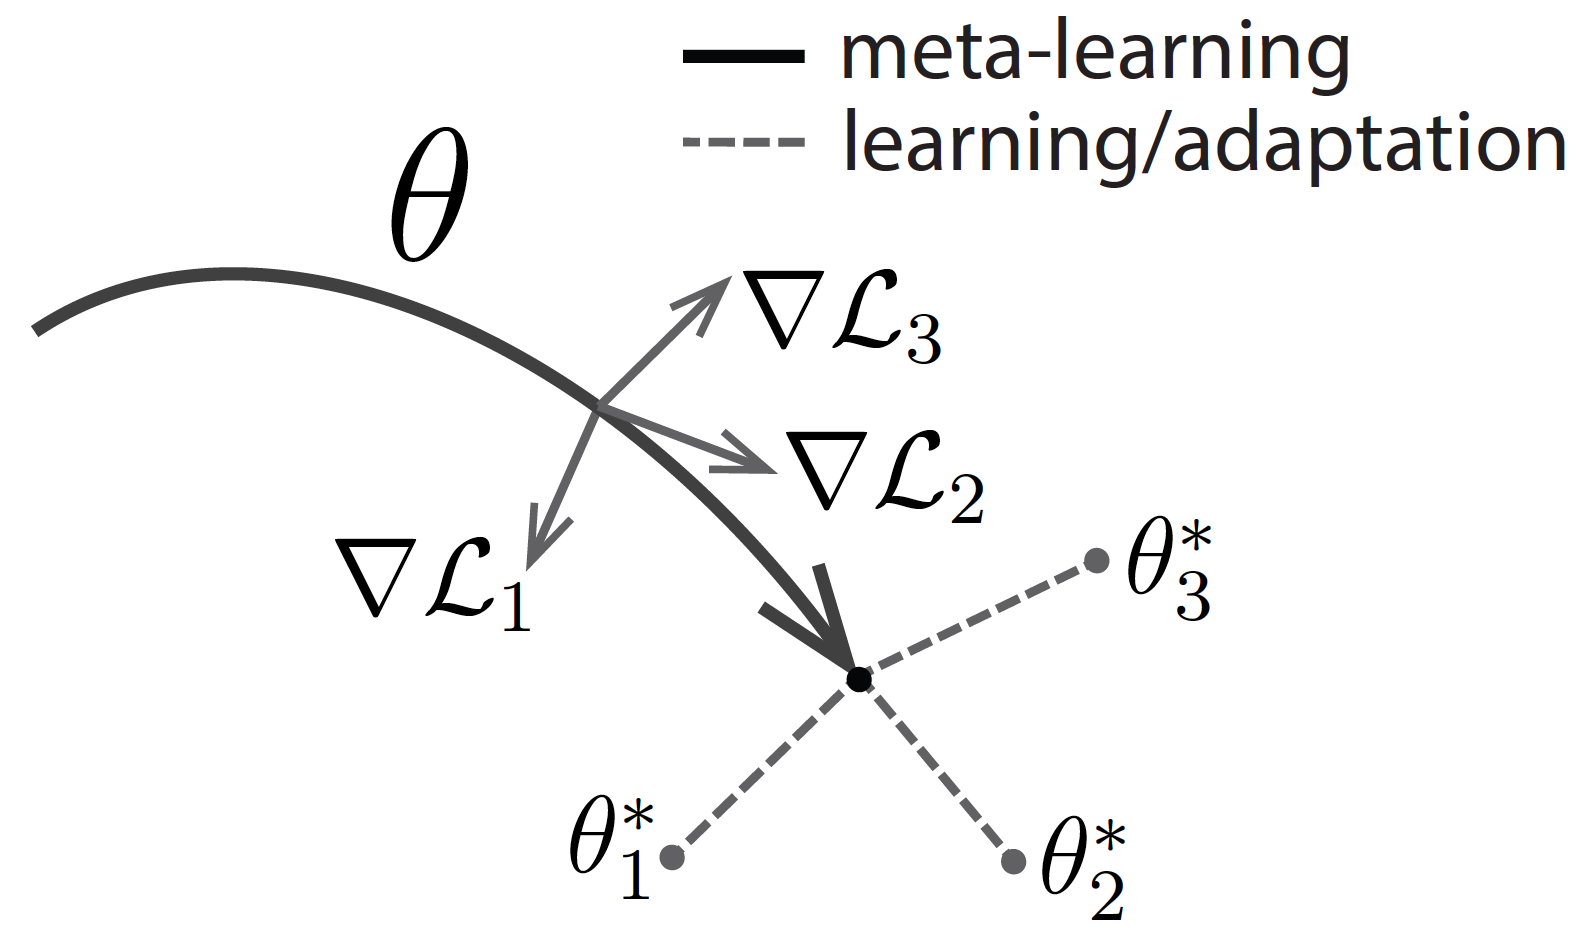
\includegraphics[width=0.45\textwidth]{media/literature/maml.png}
\caption[Diagram of a \gls{MAML} algorithm]{The figure above illustrates the \Gls{MAML} algorithm (\cite{finn_model-agnostic_2017})
}
\label{fig:MAML}
\end{figure}


Despite the primary focus of \acrshort{MAML} research relating to object recognition, it can be applied to a variety of machine learning problems with any number of training steps or data because the algorithm still produces a weight initialisation, meaning no additional learning parameters are required.

% as shown below in Figure ~\ref{fig:MAML}.
% goal of meta learning is to train model on variety of tasks 
% so that it can solve new tasks w/ small number of training samples

% In MAML, parameters of the model are trained such that a small number of gradient steps
% with a small amount of training data from a new task will produce good generalisation performance on that task

% Essentially, trains the model to be easy to fine-tune 
%
% Leads to state-of-the-art-performance with few-shot image classification benchmarks
%

% say how this paper uses meta agnostic model for translation
Research by \cite{gu_meta-learning_2018} is the first of its kind to use \acrshort{MAML} for \acrshort{NMT}. In comparison to the transfer based approach by \cite{zoph_transfer_2016}, results showed further improvements with a BLEU score of 22.04, despite training data for the low-resource language limited to 16,000 words (around 600 parallel sentences). As the corpus size of the low-resource language decreases, transfer learning approaches suffer significantly more than meta learning which proves the effectiveness for low-resource languages. However, this also means that as the corpus size increases, the difference between the two approaches becomes much less significant.


\clearpage

\section{Conclusion}
%Nulla fringilla eu eros nec tempor. Phasellus volutpat nulla a lectus pulvinar, sit amet maximus ex semper. Fusce sagittis ligula magna, non condimentum lectus imperdiet ut. Nunc dignissim turpis nibh, vel tristique tellus tristique eu. Fusce posuere dictum ultricies. Nam a metus quis mauris gravida laoreet. 